\documentclass{article}
\usepackage[utf8]{inputenc}
\usepackage{graphicx}
\usepackage{tikz}
\usepackage{listings}
\usepackage{xcolor}

\definecolor{codegreen}{rgb}{0,0.6,0}
\definecolor{codegray}{rgb}{0.5,0.5,0.5}
\definecolor{codepurple}{rgb}{0.58,0,0.82}
\definecolor{backcolour}{rgb}{0.95,0.95,0.92}

\lstdefinestyle{mystyle}{
    backgroundcolor=\color{backcolour},   
    commentstyle=\color{codegreen},
    keywordstyle=\color{magenta},
    numberstyle=\tiny\color{codegray},
    stringstyle=\color{codepurple},
    basicstyle=\ttfamily\footnotesize,
    breakatwhitespace=false,         
    breaklines=true,                 
    captionpos=b,                    
    keepspaces=true,                 
    numbers=left,                    
    numbersep=5pt,                  
    showspaces=false,                
    showstringspaces=false,
    showtabs=false,                  
    tabsize=2
}

\lstset{style=mystyle}
\renewcommand{\lstlistingname}{Algoritmo}

\title{Numeros Primos}
\author{Dueñas Jiménez Cristian Alexis}

\begin{document}
\maketitle

\section{Introducción}
El programa debe de preguntar si quiere calcular otra "n" o no y salir hasta que se le especifique. La salida debe ser expresada en notación de conjunto, debe ir a un archivo de texto. En un archivo especificar el conjunto en binario y en otro el conjunto en decimal. Del archivo de salida, graficar el número símbolos y de 1s de cada cadena. El eje de las "x" es la cadena y el eje de las "y" los símbolos que tiene esa cadena. Específicamente en el reporte, calcular y graficar cuando $n=200^3$. Al mismo tiempo, calcular adicionalmente sus logaritmo en base 10.


\section{Marco Teórico}
Los números primos son aquellos que solo son divisibles entre ellos mismos y el 1, es decir, que si intentamos dividirlos por cualquier otro número, el resultado no es entero. Dicho de otra forma, si haces la división por cualquier número que no sea 1 o él mismo, se obtiene un resto distinto de cero.

Los números binarios son números que están dentro del sistema binario de numeración que está constituido por dos cifras 1 y 0, un sistema en el cual se escriben cantidades, códigos, mensajes y otros lenguajes con tan solo dos elementos dentro de la numeración, haciendo que el código se simplifique la comprensión de los sistemas informáticos, pues hará que un elemento tenga un valor unitario o nulo. Es decir que se trabaja en un sistema de puertas cerradas o abiertas.
\section{Desarrollo}


Primero, se hace uso de listas para guardar datos que nos serán de utilidad para posteriormente graficar nuestros datos.

\begin{lstlisting}[language=Python, caption=Números primos hasta N]
import numpy as np
from functions import *
import sys

def getPrimos(n):
    primos = []
    unos = []
    largo =[]
    cont = -1

    f_primo1 = open("../PARCIAL 1/PROGRAMAS/Programa2/outputs/primosbin.txt", "w", encoding="utf-8")
    f_primo2 = open("../PARCIAL 1/PROGRAMAS/Programa2/outputs/primosint.txt", "w", encoding="utf-8")

    f_primo1.write("{ε")
    f_primo2.write("{ε")
    for i in range (2,n+1):
        if Primo(i):
            primos.append(i)
            binario = bin(i)[2:]
            f_primo1.write(','+binario)
            cont+=1
            f_primo2.write(','+str(i))    
            unos.append(binario.count('1'))
            largo.append(cont) 
    
    f_primo1.write("}")
    f_primo2.write("}")
    f_primo1.close()
    f_primo2.close()
    graficar(largo, unos, "Cadenas", "Cantidad de 1's")
    graficar(largo, np.log10(unos), "Cadenas", "Cantidad de 1's (Log10)")
    graficar(largo, np.log2(unos), "Cadenas", "Cantidad de 1's (Log2)")

#Generamos nuestro menú de opciones
opc = "1"
print("MENU DE OPCIONES")
while opc == "1":
    
    opc = input("Seleccione una opción: \n1.- Ingresar n \n2.- Finalizar\n")
    
    if opc == "1":
        n = int(input("Ingrese el valor de n: "))
        getPrimos(n)
    else:
        if opc == "2":
            print(f"FIN DE LA EJECUCION")
            sys.exit(0)
        else:
            if opc != "1":
                print("Seleccione una opcion valida")

\end{lstlisting}

\begin{lstlisting}[language=Python, caption=Funciones para la clase main]
import matplotlib.pyplot as plt

def graficar(largo, unos, ejeX, ejeY):
    
    plt.plot(largo, unos, marker="")
    plt.xlabel(ejeX)
    plt.ylabel(ejeY)
    plt.title("GRAFICA")
    plt.show()

def Primo(num):
    bandera = False
    if num > 1:  
        for j in range(2, int(num/2) + 1):  
            if (num % j) == 0:
                break  
        else:  
            bandera = True     
    return bandera
\end{lstlisting}

Lo que hacemos es crear una función que determine cuando un número es Primo o no es primo. Si es el caso de que sí, retorna verdadero, y en caso de que no, retorna falso. Posteriormente utilizamos la función sigma, la cual recibe un valor "n" y este delimita de donde a donde se buscarán  números primos.  
\newline\newline
Para esto creamos 2 archivos, uno con el nombre de primosbin y otro con el nombre de primosint, ambos de tipo txt y estos almacenarán según sea el caso, el número primo encontrado.
Generamos un bucle que va empieza desde 2, ya que de lo contrario tomaría al 1 como primo y no pertenece a esa familia. Realiza la comparación con cada uno de los valores , llamando a la función Primo y mandandole el valor de la posición en la que va nuestro for. Cada que sea primo, lo convierte a binario y se mandan a escribir a cada uno de los archivos según correspondan.
\newline\newline
Para graficar, hacemos uso de la librería matplotlib. El programa tiene una función en onde recibe los arreglos llenados en la función sigma, que usa para representarlos en la gráfica. 


\subsection{Implementación}
\begin{center}
    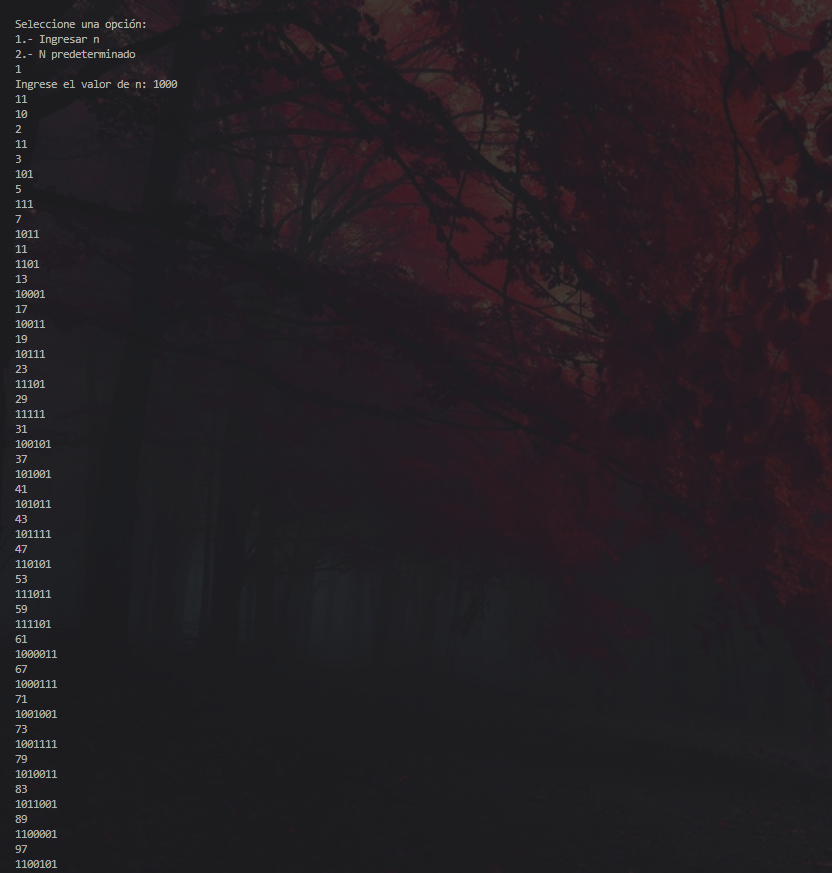
\includegraphics[scale = 0.5]{TestSistema.PNG}
    \caption{Consola}
\end{center}

\begin{center}
    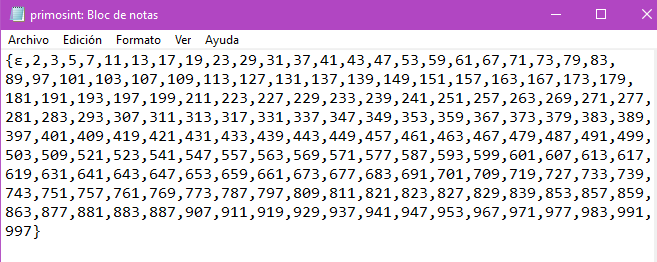
\includegraphics[scale = 0.7]{primostest2.png}
\end{center}

\begin{center}
    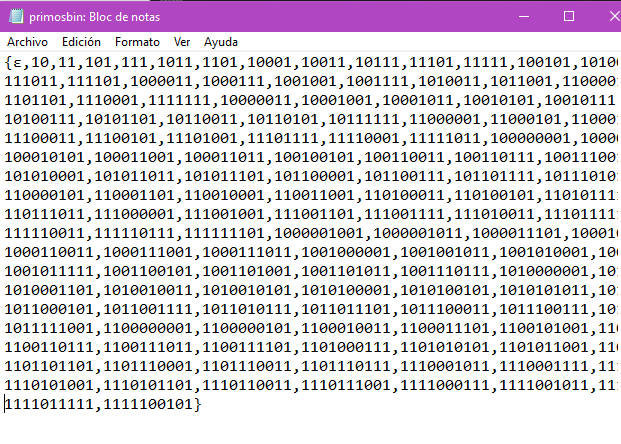
\includegraphics[scale = 1.5]{primostest3.PNG}
\end{center}

\begin{center}
    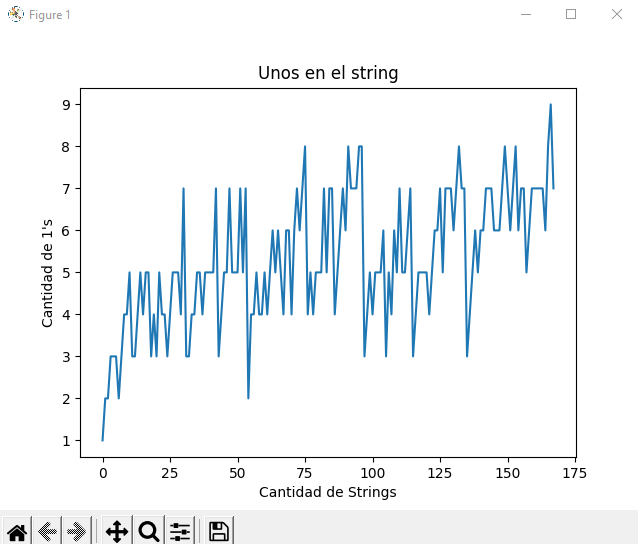
\includegraphics[scale = 0.7]{Grafica.png}
    \caption{Grafica 1}
\end{center}

\begin{center}
    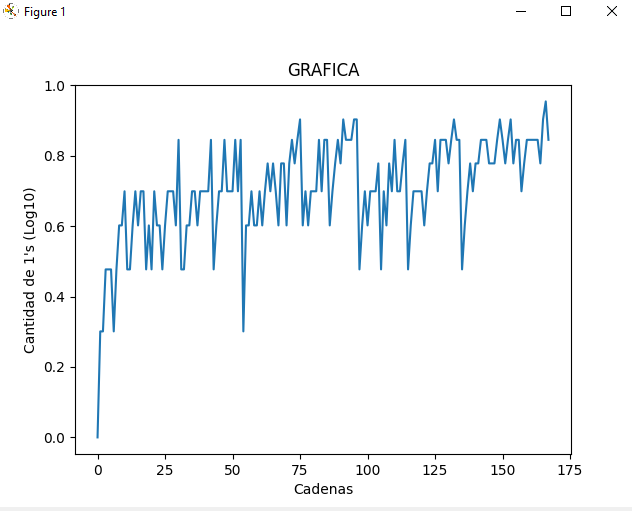
\includegraphics[scale = 0.7]{Graphic2.png}
    \caption{Grafica 2}
\end{center}

\begin{center}
    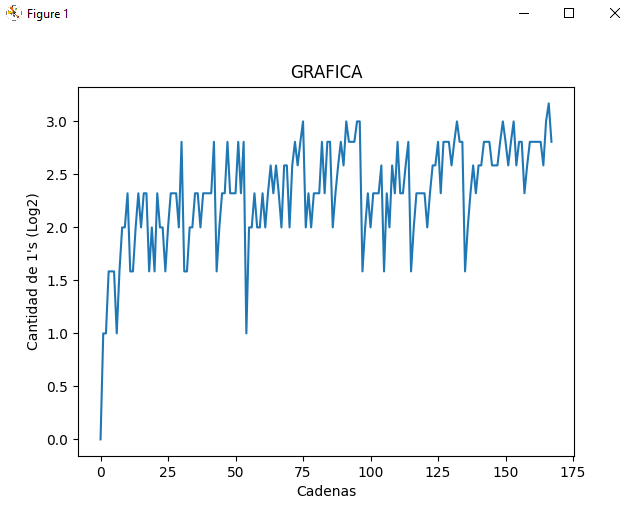
\includegraphics[scale = 0.7]{Graphic3.png}
    \caption{Grafica 3}
\end{center}

\section{Conclusión}
Con la realización de este ejercicio, podemos ver que un trabajo que parece bastante complejo se puede resumir a breves líneas de código. Uno pensaría que para calcular la cantidad de números primos que hay de 1 a una cantidad inmensa es bastante tedioso, claramente si nos ponemos a hacerlo a mano sí, pero utilizando nuestro conocimientos podemos generar cosas como este ejercicio, que bien es cierto que no va a calcular los números primos hasta infinito, pero sí a una cantidad que para nosotros sería de mucho tiempo.
\newline
\newline
\newline
\newline
\newline
\newline
\newline
\begin{thebibliography}{}
    \bibitem{automata}
    Rivera, C. (2022, 14 marzo). Números primos y compuestos: qué son + ejemplos. Smartick. Recuperado 19 de junio de 2022, de https://www.smartick.es/blog/matematicas/numeros-enteros/numeros-primos-y-numeros-compuestos/#:%7E:text=Los%20n%C3%BAmeros%20primos%20son%20aquellos,un%20resto%20distinto%20de%20cer
\end{thebibliography}

\end{document}